\documentclass[conf]{new-aiaa}
%\documentclass[journal]{new-aiaa} for journal papers
\usepackage[utf8]{inputenc}

\usepackage{graphicx}
\usepackage{amsmath}
\usepackage{commath}
\usepackage[version=4]{mhchem}
\usepackage{siunitx}
\usepackage{longtable,tabularx}
\usepackage{float}
\usepackage{listings}
\usepackage{pdfpages}
\usepackage{color} %red, green, blue, yellow, cyan, magenta, black, white
\definecolor{mygreen}{RGB}{28,172,0} % color values Red, Green, Blue
\definecolor{mylilas}{RGB}{170,55,241}
\setlength\LTleft{0pt} 

\lstset{language=Matlab,%
	basicstyle=\footnotesize,
	breaklines=true,%
	morekeywords={matlab2tikz},
	keywordstyle=\color{blue},%
	morekeywords=[2]{1}, keywordstyle=[2]{\color{black}},
	identifierstyle=\color{black},%
	stringstyle=\color{mylilas},
	commentstyle=\color{mygreen},%
	showstringspaces=false,%without this there will be a symbol in the places where there is a space
	numbers=left,%
	numberstyle={\tiny \color{black}},% size of the numbers
	numbersep=9pt, % this defines how far the numbers are from the text
	emph=[1]{for,end,break},emphstyle=[1]\color{red}, %some words to emphasise
	%emph=[2]{word1,word2}, emphstyle=[2]{style},    
}

% ================================================================ % 
\title{ASE 389P.4 Methods of Orbit Determination \\ Homework 3: The Batch and Sequential Processor}

\author{Junette Hsin}
\affil{Masters Student, Aerospace Engineering and Engineering Mechanics, University of Texas, Austin, TX 78712}

\begin{document}

\maketitle

\begin{abstract}
	The numeric propagation of the state transition matrix (STM) and the batch processor were explored. A state transition matrix (STM) for a two-dimensional, two-body orbit was first generated and verified by comparing the mapped deviations to differences in the nonlinear solution. Finally, a nonlinear batch processor and the sequential processor for a simple problem were implemented.


\end{abstract}


% ================================================================ % 
\section*{Problem 1}

 % \subsubsection*{Statement} 
\begin{center}
\fbox{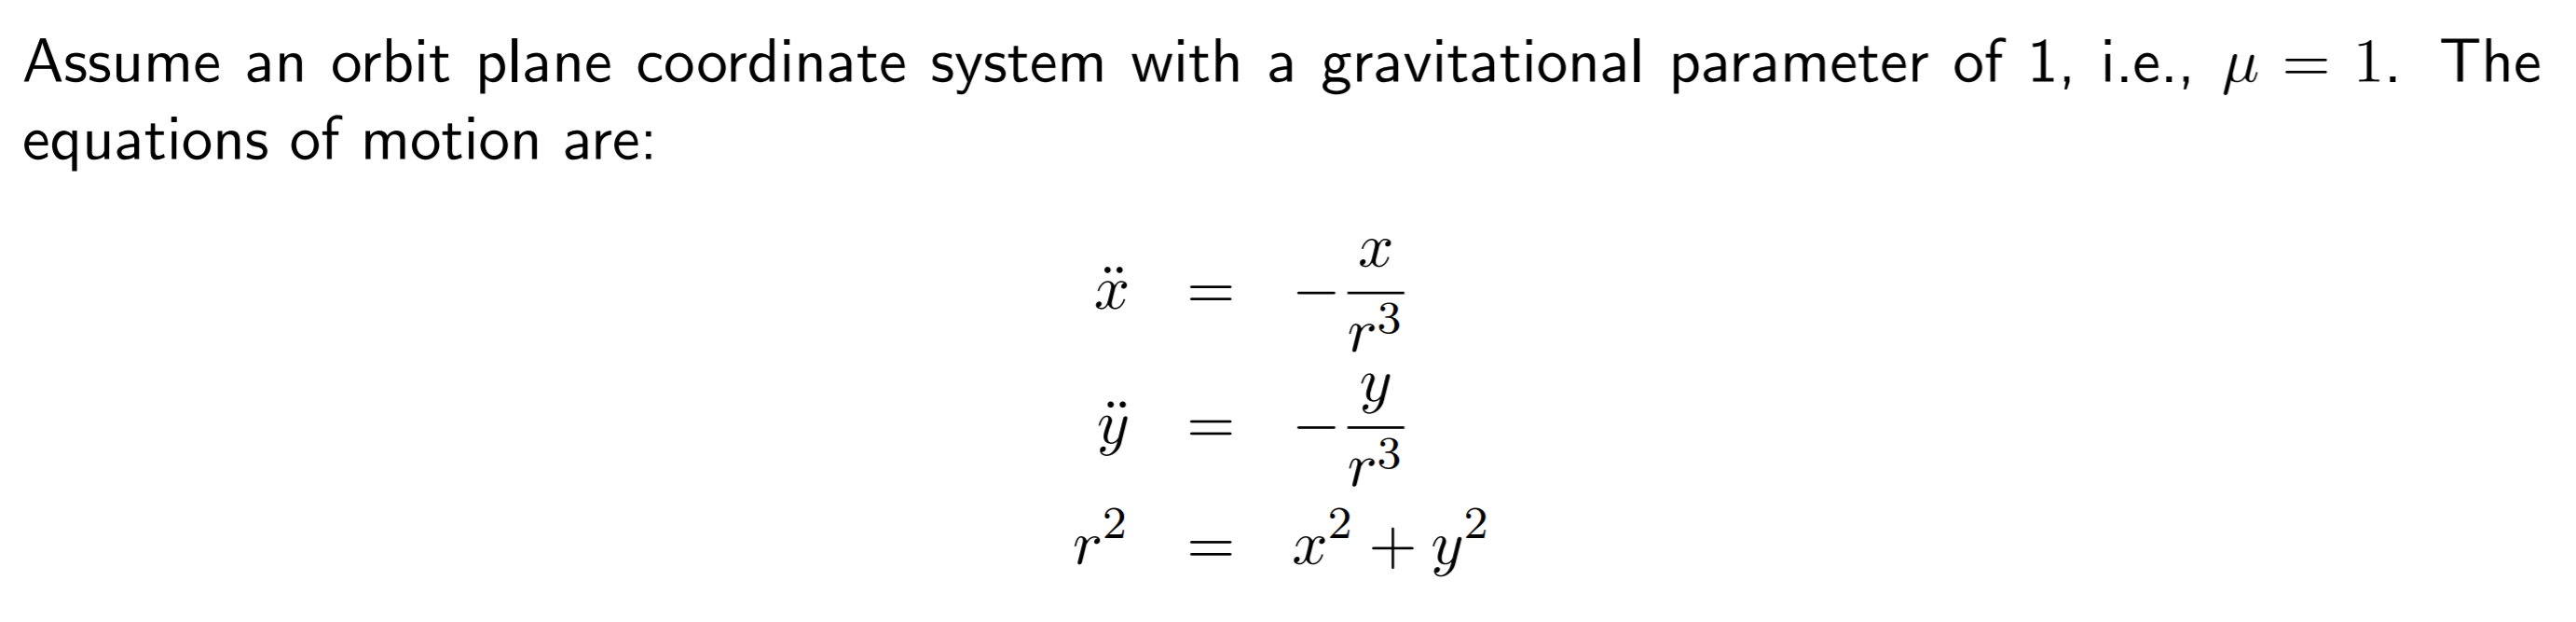
\includegraphics[width=0.9\textwidth]{prob_1.png}} \\
\end{center}

% ---------------------------------------------------------------- % 
%\subsubsection*{Solution} 

% ... 

%\newpage
% ================================================================ % 

\subsection*{Problem 1a} 

 % \subsubsection*{Statement} 
\begin{center}
	\fbox{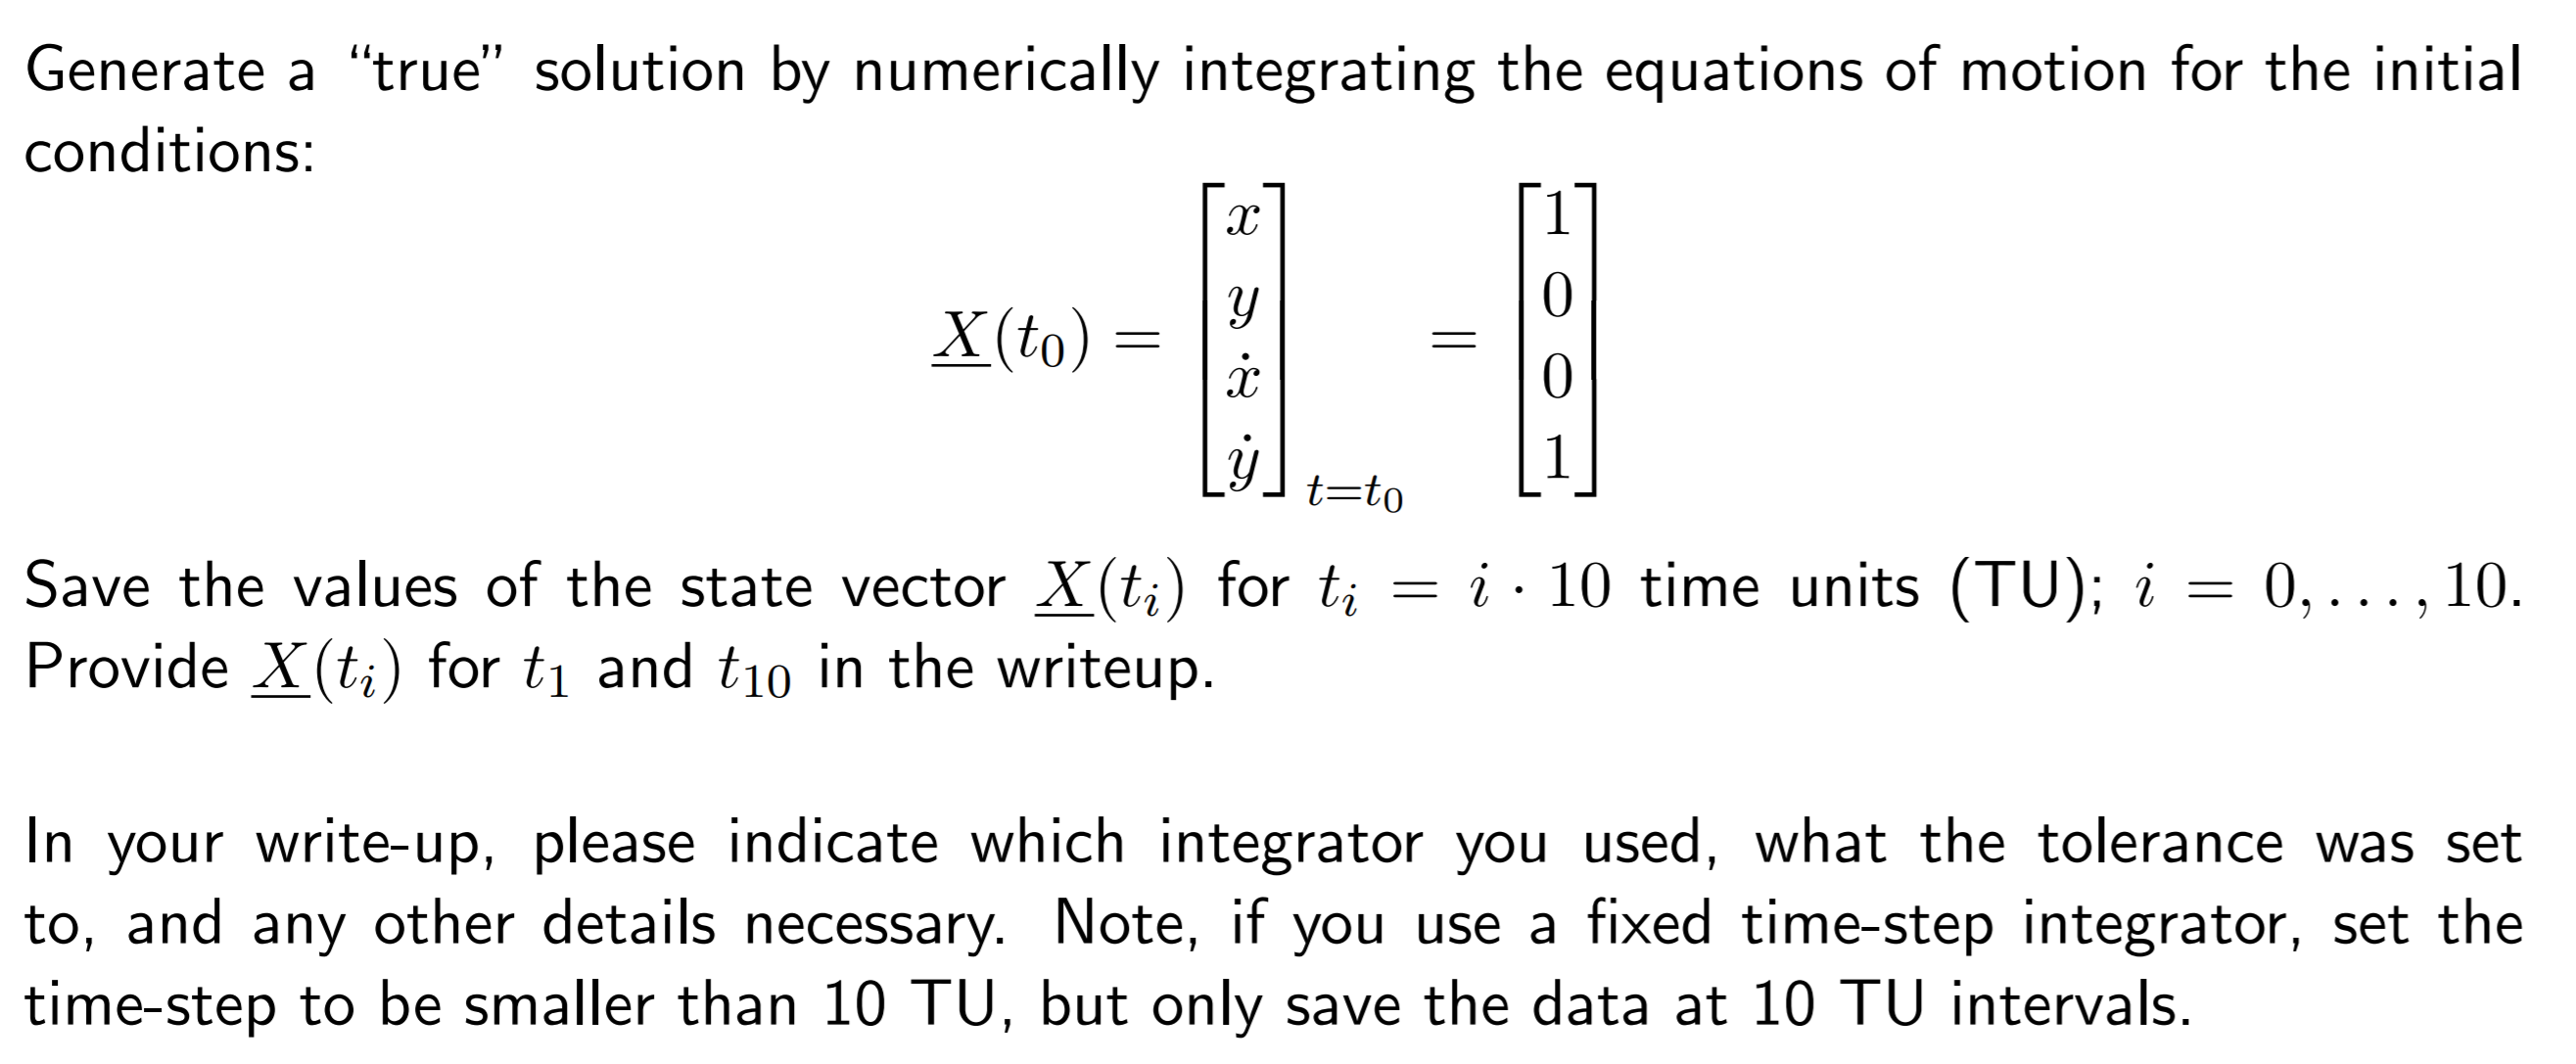
\includegraphics[width=0.9\textwidth]{prob_1a.png}} \\
\end{center}

% ---------------------------------------------------------------- % 

\subsubsection*{Solution} 

\begin{equation}
	\underline{X}(t_1) = [         -0.839071529076614,~        -0.544021110889203,~         0.544021110889159,~        -0.839071529076556 ]^T
\end{equation}

\begin{equation}
	\underline{X}(t_{10}) = [ 0.862318872276158,~        -0.506365641129975,~         0.506365641129749,~         0.862318872275784 ]^T
\end{equation}


\texttt{ode45} was used to integrate with the relative tolerance set to 3e-14 and absolute tolerance set to 1e-16. The time step was 10 ms, or 100 Hz. 


%\begin{lstlisting}
%% set ode45 params 
%rel_tol = 3e-14;         % 1e-14 accurate; 1e-6 coarse 
%abs_tol = 1e-16; 
%options = odeset('reltol', rel_tol, 'abstol', abs_tol ); 
%
%rv0 = [1; 0; 0; 1]; 
%dt = 0.01; 
%
%% integrate 
%[t, rv] = ode45(@fn.TwoBod_4states, [0:dt:100], [rv0], options); 
%\end{lstlisting}


\newpage
% ================================================================ % 

\subsection*{Problem 1b} 

% \subsubsection*{Statement} 
\begin{center}
	\fbox{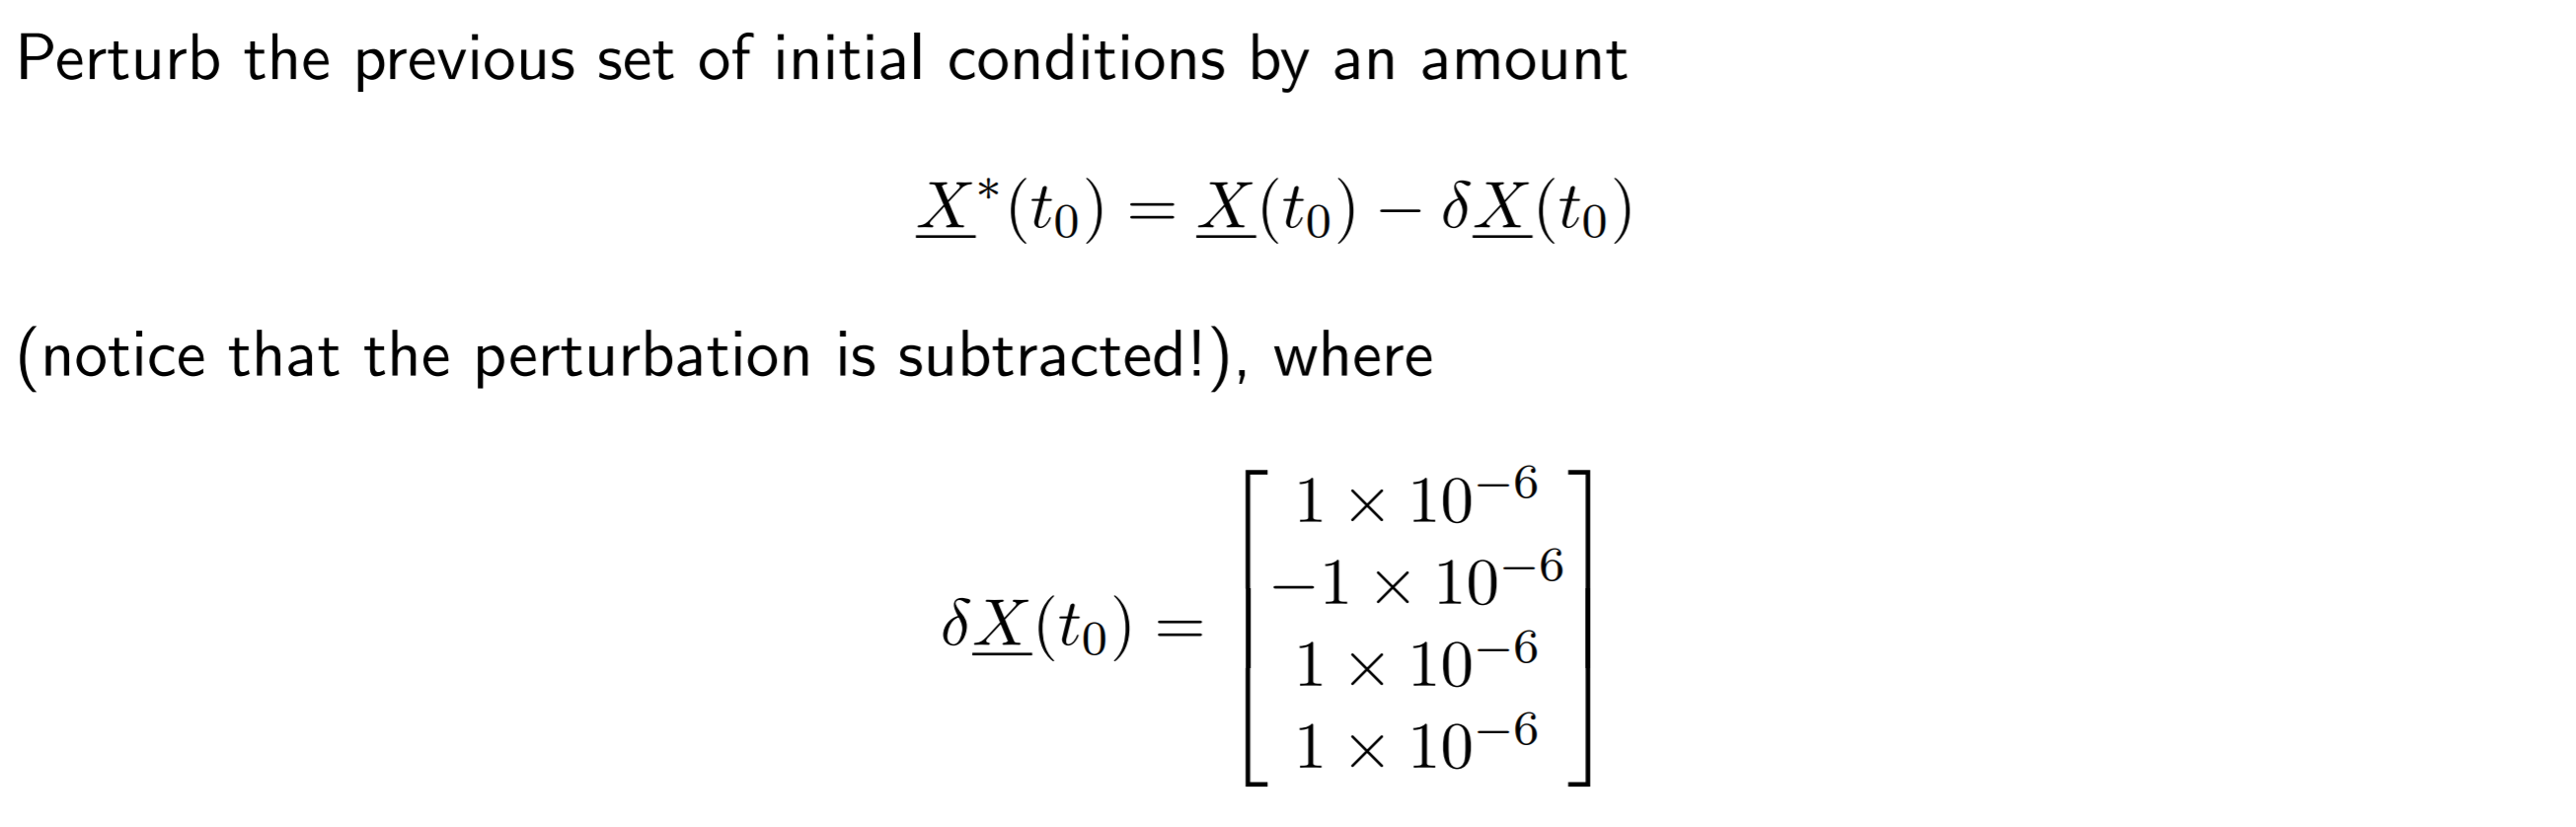
\includegraphics[width=0.9\textwidth]{prob_1b.png}} \\
	\fbox{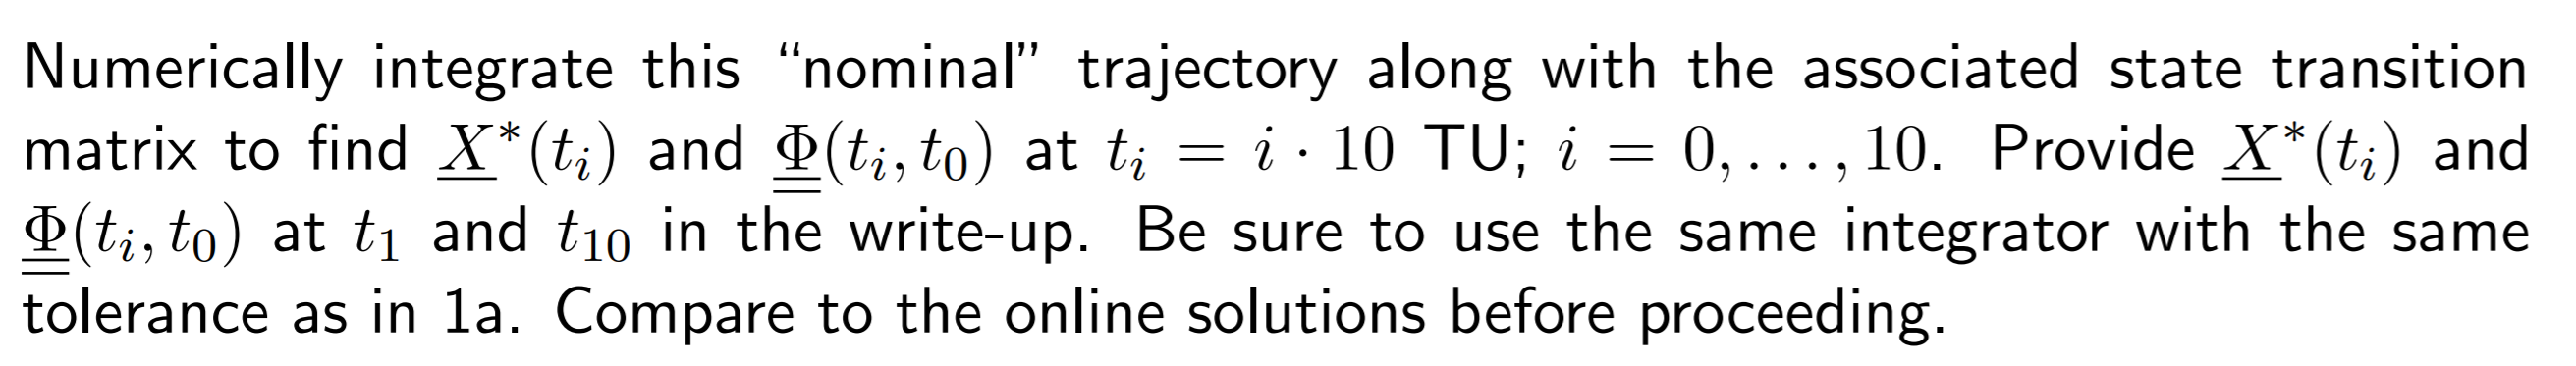
\includegraphics[width=0.9\textwidth]{prob_1b_2.png}} \\
\end{center}

% ---------------------------------------------------------------- % 

\subsubsection*{Solution} 

Note: For the solutions in this homework, $\Phi$ will be used to represent $\underline{\underline{\Phi}}$ to stay consistent with the convention used in the text, particularly for Problem 1c. 

\begin{equation}
	\underline{X}^*(t_{1}) = [         -0.839031098038944,~
	-0.544071486479261,~
	0.544076120415627,~
	-0.839041244186316 ]^T
\end{equation}

\begin{equation}
	\Phi(t_{1}, t_0) = 
	\begin{bmatrix}
         -19.2963174705313    &     -1.00059195284582    &     -1.54462409476518   &       -20.592274677963 \\
		24.5395368984514      &    2.54304003750491      &    3.38202243902567     &     24.9959638292643 \\
		-26.628448580308      &   -1.24704108018372      &    -2.0860289935347     &    -27.5413748340174 \\
		-15.0754226453647     &    -1.45709728481153     &    -2.00114420643928    &     -14.6674122499641
	\end{bmatrix}
\end{equation}

\begin{equation}
	\underline{X}^*(t_{10}) = [          0.862623359653583,~
	-0.505843963221603,~
	0.50584568923193,~
	0.862623303038346 ]^T
\end{equation}

\begin{equation}
	\Phi(t_{10}, t_0) = 
	\begin{bmatrix}
         -151.284032326374   &    -0.0696433460453671   &     -0.575183991319675   &      -152.539455288431 \\
		-260.234514431179    &     0.881235606618973    &    0.0191322894654827    &     -260.670088444015 \\
		259.154447538201     &    0.374643452779477     &     1.23674843709451     &     260.026380249705 \\
		-152.127910765101    &     0.366712857375205    &    -0.138829570274937    &     -151.639213163376
	\end{bmatrix}
\end{equation}


\newpage
% ================================================================ % 

\subsection*{Problem 1c} 

% \subsubsection*{Statement} 
\begin{center}
	\fbox{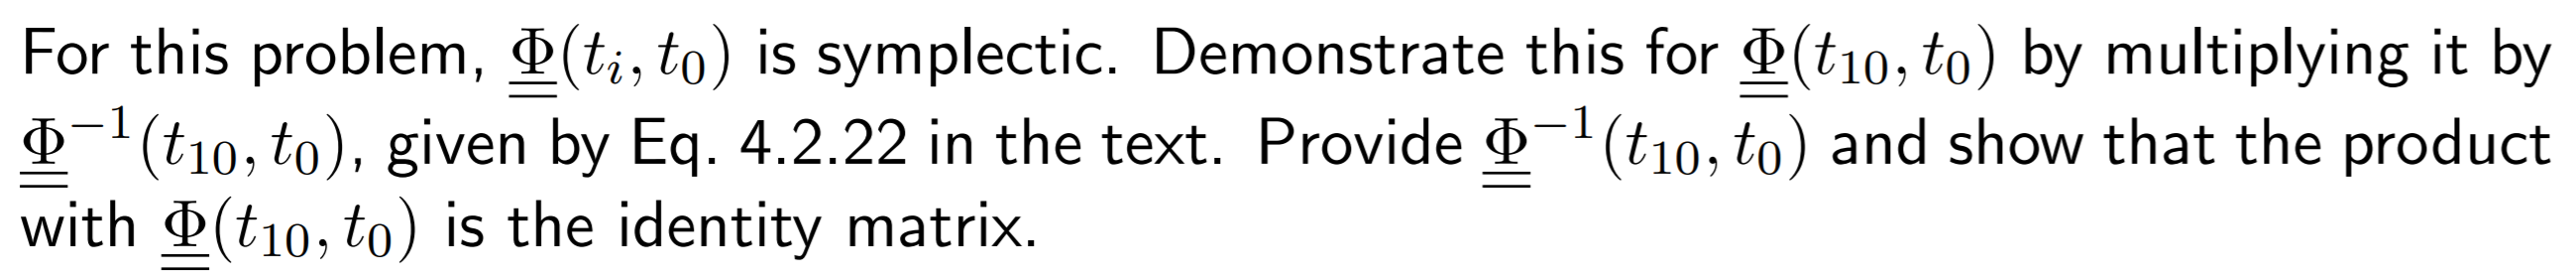
\includegraphics[width=0.9\textwidth]{prob_1c.png}} \\
\end{center}

% ---------------------------------------------------------------- % 

\subsubsection*{Solution} 

From Eq. 4.2.22 in the text\cite{born_statorbitdet}: 

\begin{equation}
	\Phi^{-1}(t, t_k) = 
	\begin{bmatrix}
		\Phi^T_4 & -\Phi^T_2 \\ 
		-\Phi^T_3 & \Phi^T_1
	\end{bmatrix}
\end{equation}

From $\Phi( t_{10}, t_0 )$ in Problem 1b, $\Phi^T_4, \Phi^T_2, \Phi^T_3$ and $\Phi^T_1$ are as follows: 

\begin{equation}
	\Phi^T_1 = 
	\begin{bmatrix}		
		-151.284032326374   &    -0.0696433460453671    \\
		-260.234514431179    &     0.881235606618973    
	\end{bmatrix}
\end{equation}

\begin{equation}
	\Phi^T_2 = 
	\begin{bmatrix}
		-0.575183991319675   &      -152.539455288431 \\
	 	0.0191322894654827    &     -260.670088444015 
	\end{bmatrix}
\end{equation}

\begin{equation}
	\Phi^T_3 = 
	\begin{bmatrix}
		259.154447538201     &    0.374643452779477      \\
		-152.127910765101    &     0.366712857375205    
	\end{bmatrix}
\end{equation}

\begin{equation}
	\Phi^T_4 = 
	\begin{bmatrix}
		1.23674843709451     &     260.026380249705 \\
		-0.138829570274937    &     -151.639213163376
	\end{bmatrix}
\end{equation}

The inverse of $\Phi( t_{10}, t_0 )$ evaluates to: 

\begin{equation}
	\Phi^{-1}(t_{10}, t_0) = 
	\begin{bmatrix}
		1.23674843709451    &    -0.138829570274937     &    0.575183991319675    &   -0.0191322894654827 \\
		260.026380249705    &     -151.639213163376     &     152.539455288431    &      260.670088444015 \\
		-259.154447538201   &       152.127910765101    &     -151.284032326374   &      -260.234514431179 \\
		-0.374643452779477  &      -0.366712857375205   &    -0.0696433460453671  &       0.881235606618973
	\end{bmatrix}
\end{equation}

The product of $\Phi^{-1}(t_{10}, t_0)$ and $\Phi(t_{10}, t_0)$ is the identity matrix, which shows that $\Phi(t_{10}, t_0)$ is symplectic. The format is short so that the significant figures may fit on the page: 

\begin{equation}
	\Phi^{-1}(t_{10}, t_0) \Phi(t_{10}, t_0) = \\
	\begin{bmatrix}
%		0.99999999999392   &   -5.8866973795535e-14  &    2.03830008427275e-17  &   -1.00635055844123e-11 \\
%		9.45874489843845e-11    &      1.00000000000514   &   1.00541797110054e-11   &                      0 \\
%		0  &   -1.77635683940025e-12    &     0.999999999993904   &   9.45874489843845e-11 \\
%		1.79056769411545e-12            &             0   &  -5.88556980929411e-14     &     1.00000000000514
				
		1.0000 &  -0.0000 &   0.0000 &  -0.0000 \\
		0.0000 &   1.0000 &   0.0000 &        0 \\
		0  & -0.0000 &   1.0000 &   0.0000      \\
		0.0000 &        0 &  -0.0000 &   1.0000
		
	\end{bmatrix}
\end{equation}


\newpage
% ================================================================ % 

\subsection*{Problem 1d} 

% \subsubsection*{Statement} 
\begin{center}
	\fbox{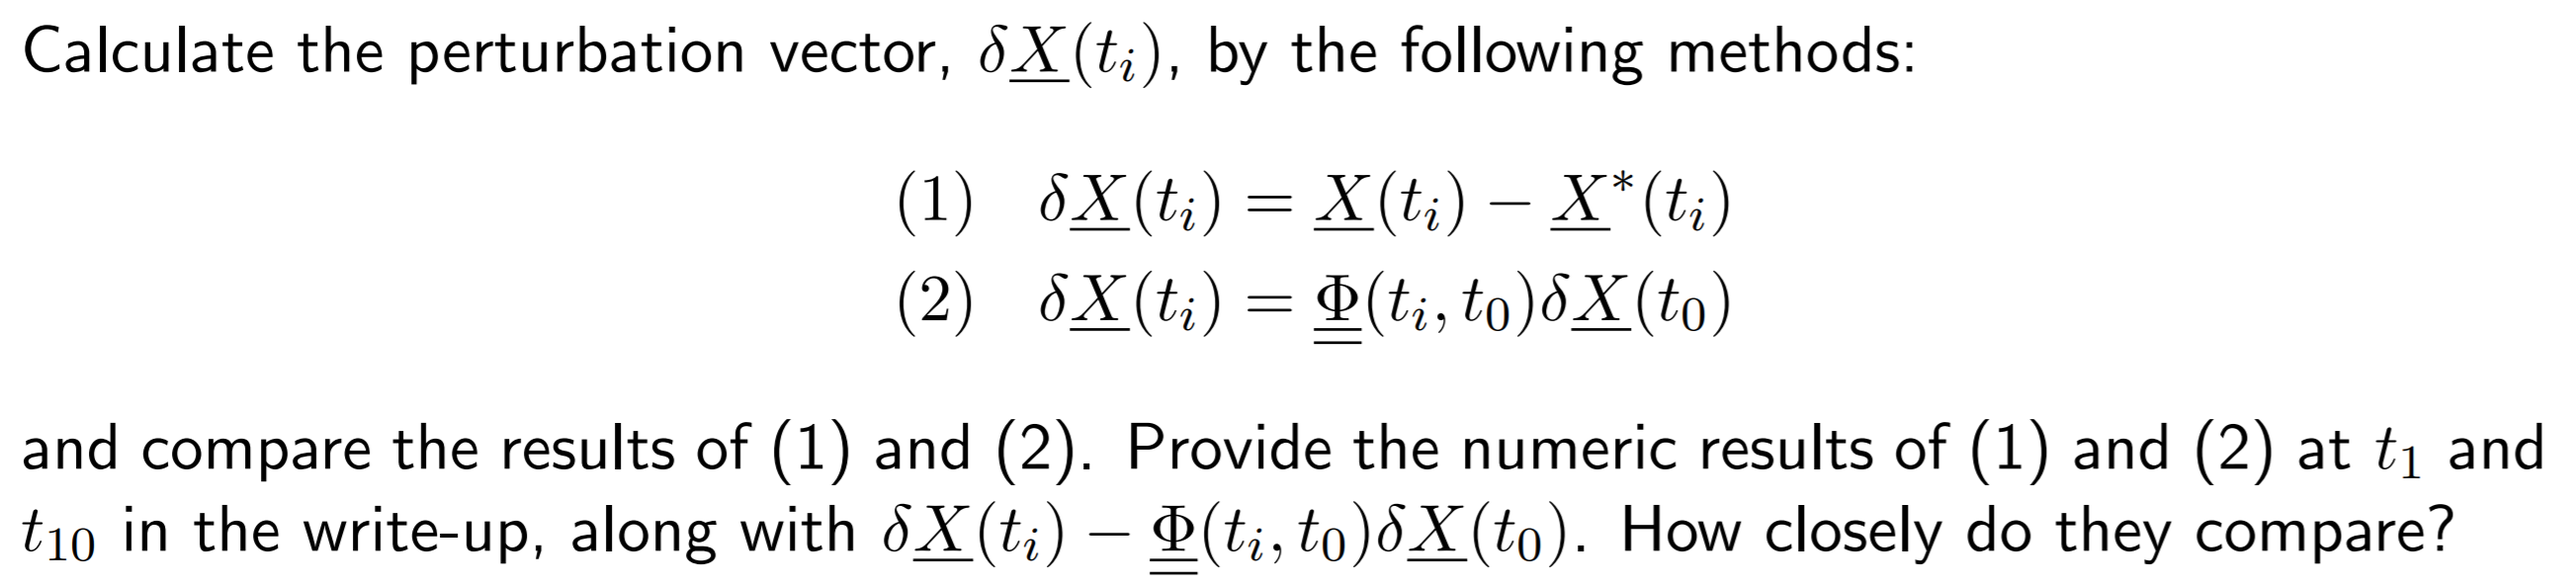
\includegraphics[width=0.9\textwidth]{prob_1d.png}} \\
\end{center}

% ---------------------------------------------------------------- % 

\subsubsection*{Solution} 

$\delta \underline{X}(t_1)$ from method 1: 

\begin{equation}
	\delta \underline{X}(t_1) = 
	\begin{bmatrix}
		-4.04310376698191e-05 \\
		5.03755900577163e-05 \\
		-5.5009526467753e-05 \\
		-3.02848902397068e-05 		
	\end{bmatrix}
\end{equation}

$\delta \underline{X}(t_1)$ from method 2: 

\begin{equation}
	\delta \underline{X}(t_1) = 
	\begin{bmatrix}
		-4.04326242904136e-05 \\
		5.03744831292364e-05 \\
		-5.50088113276763e-05 \\
		-3.02868818169565e-05
	\end{bmatrix}
\end{equation}

The difference between the two methods for $\delta \underline{X}(t_1)$ is the following: 

\begin{equation}
	\begin{bmatrix}
		1.58662059446919e-09 \\
		1.10692847990051e-09 \\
		-7.15140076693879e-10 \\
		1.99157724972097e-09
	\end{bmatrix}
\end{equation}

$\delta \underline{X}(t_{10})$ from method 1: 

\begin{equation}
\delta \underline{X}(t_{10}) = 
\begin{bmatrix}
     -0.000304487377425611 \\
	-0.000521677908372098 \\
	0.000519951897818727 \\
	-0.000304430762562036
\end{bmatrix}
\end{equation}

$\delta \underline{X}(t_{10})$ from method 2: 

\begin{equation}
\delta \underline{X}(t_{10}) = 
\begin{bmatrix}
     -0.000304329028260079 \\
	-0.000521766706192347 \\
	0.000520042932772221 \\
	-0.000304272666356127
\end{bmatrix}
\end{equation}

The difference between the two methods for $\delta \underline{X}(t_{10})$ is the following: 

\begin{equation}
	\begin{bmatrix}
	     -1.58349165531931e-07 \\
		8.8797820249403e-08 \\
		-9.10349534938987e-08 \\
		-1.5809620590901e-07
	\end{bmatrix}
\end{equation}

$t_{10}$ is 10 TU larger than $t_1$, but the order of magnitude of the difference between both methods increases by 2 from $t_1$ to $t_{10}$. The results from both methods are quite close, but gradually diverge as time goes on. 


%\newpage
% ================================================================ % 

\section*{Problem 2} 

% \subsubsection*{Statement} 
\begin{center}
	\fbox{
\includegraphics[width=0.9\textwidth]{prob_2.png}} \\
\end{center}

% ---------------------------------------------------------------- % 

%\subsubsection*{Solution} 


%\newpage
% ================================================================ % 

\subsection*{Problem 2a} 

% \subsubsection*{Statement} 
\begin{center}
	\fbox{
\includegraphics[width=0.9\textwidth]{prob_2a.png}} \\
\end{center}

% ---------------------------------------------------------------- % 

\subsubsection*{Solution} 

\begin{equation}
	\hat{x} = 1.5
\end{equation}

The method employed in the code is the following: 

1. Given $\underline{y}, \underline{\underline{W}}$, and $\underline{\underline{H}}$, and \emph{a priori} information $\bar{x}$ and $\bar{W}$, 

2. Initialize $\Lambda = \bar{W}$

3. Initialize $N = \bar{W} \bar{x}$

4. Accumulate $\Lambda = \Lambda + \underline{\underline{H}}^T \underline{\underline{W}} ~ \underline{\underline{H}}$

5. Accumulate $ N = N + \underline{\underline{H}} ~ \underline{\underline{W}} ~\underline{y} $

6. Use the normal equation to find $\hat{x}$ (multiply both sides by inverted $\Lambda$): $\Lambda \hat{x} = N$

%The snippet of code used to solve Problem 2a is below: 
%
%\begin{lstlisting}
%	% observation states & a priori info 
%	y = [1; 2; 1]; 
%	W = [2 0 0; 0 1 0; 0 0 1]; 
%	H = [1; 1; 1]; 
%	x0 = 2; 
%	W0 = 2; 
%	
%	% Lambda = inv(P) = W0  
%	P0      = inv(W0); 
%	Lambda  = W0; 
%	R       = inv(W); 
%	
%	% N = inv(P) * x0 = W0 * x0 
%	N = W0 * x0; 
%	
%	% accumulate 
%	Lambda  = Lambda + H' * W * H; 
%	N       = N + H' * W * y; 
%	
%	% normal equation 
%	xhat = inv(Lambda) * N; 
%\end{lstlisting}


%\newpage
% ================================================================ % 

\subsection*{Problem 2b} 

% \subsubsection*{Statement} 
\begin{center}
	\fbox{
\includegraphics[width=0.9\textwidth]{prob_2b.png}} \\
\end{center}

% ---------------------------------------------------------------- % 

\subsubsection*{Solution} 

The error can be found from the observation state relation: 

\begin{equation}
	e = \underline{y} - \underline{\underline{H}} \hat{x}
\end{equation}

The best estimate of the observation error is: 

\begin{equation}
	e = [-0.5, 0.5, -0.5]^T 
\end{equation}






%\newpage
% ================================================================ % 
\section*{Appendix} 



%\newpage
\subsection*{HW3 MATLAB code} 

\begin{lstlisting}[basicstyle=\footnotesize]
% ASE 389 Orbit Determination
% HW 2
% Junette Hsin 

clear; 

%% Problem 1a: 

global mu 
mu = 1; 

% set ode45 params 
rel_tol = 3e-14;         % 1e-14 accurate; 1e-6 coarse 
abs_tol = 1e-16; 
options = odeset('reltol', rel_tol, 'abstol', abs_tol ); 

rv0 = [1; 0; 0; 1]; 
dt = 0.01; 

% integrate 
[t, rv] = ode45(@fn.TwoBod_4states, [0:dt:100], [rv0], options); 

%% Problem 1b: 

drv0 = [1e-6; -1e-6; 1e-6; 1e-6]; 
STM0 = eye(4); 
STM0 = reshape(STM0, [16 1]); 

rvSTM0 = [rv0 - drv0; STM0]; 

% integrate 
[tstar, rvstar] = ode45(@fn.TwoBod_4states_STM, [0:dt:100], [rvSTM0], options); 

STMf = rvstar(end, 5:20); 
STMf = reshape(STMf, [4 4]); 

%% Problem 1c: 

STMf1 = STMf(1:2, 1:2); 
STMf2 = STMf(1:2, 3:4); 
STMf3 = STMf(3:4, 1:2); 
STMf4 = STMf(3:4, 3:4); 

STMfinv = [ STMf4',  -STMf2'; ... 
-STMf3', STMf1' ]; 

STMfinv * STMf 

%% Problem 1d: 

% t1 = 10 TU
i = 10 / dt + 1; 
STMi = rvstar(i, 5:20); 
STMi = reshape(STMi, [4 4]); 

drv1 = rv(i,:) - rvstar(i,1:4); 
drv2 = STMi * drv0; 

ddrvt1 = drv1' - drv2; 

% t10 = 100 TU
i = 100 / dt + 1; 
STMi = rvstar(i, 5:20); 
STMi = reshape(STMi, [4 4]); 

drv1 = rv(i,:) - rvstar(i,1:4); 
drv2 = STMi * drv0; 

ddrvt10 = drv1' - drv2; 

%% Problem 2: Given the observation state relation y = H x + eps, where x is a scalar and
% y = [1; 2; 1]
% W = [2 0 0; 0 1 0; 0 0 1]; 
% H = [1; 1; 1]; 
% with a priori information xbar = 2 and Wbar = 2:
% 
% Problem 2a: Using the batch processing algorithm, what is x^? In the write-up, outline the method
% employed in the code.

% W matrix is inv(R) 
% Wbar = inv(P) 

% observation states 
y = [1; 2; 1]; 
W = [2 0 0; 0 1 0; 0 0 1]; 
H = [1; 1; 1]; 

x0 = 2; 
W0 = 2; 

% Lambda = inv(P) = W0  
P0      = inv(W0); 
Lambda  = W0; 
R       = inv(W); 

% N = inv(P) * x0 = W0 * x0 
N = W0 * x0; 

% accumulate 
Lambda  = Lambda + H' * W * H; 
N       = N + H' * W * y; 

% normal equation 
xhat = inv(Lambda) * N; 

e = y - H*xhat; 

%% Problem 2b: What is the best estimate of the observation error, eps? 

e = y - H*xhat; 

\end{lstlisting}

\subsection*{Two Body EOM} 
\begin{lstlisting}
function dx = TwoBod_4states(t, x)
% ------------------------------------------------------------------------
% Inputs 
%   t = [Nx1] time vector (orbit is Keplerian, doesn't matter) 
%   x = [4x1] state vector 
% 
% Outputs 
%   dx = [4x1] derivative of state vector 
% ------------------------------------------------------------------------

global mu 

dx = zeros(4, 1);   % force column vector 

% dx1 = x3 
% dx2 = x4 
% dx3 = (-u/r^3) * x1
% dx4 = (-u/r^3) * x2

dx(1:2) = x(3:4); 
r_norm  = norm(x(1:2)); 
dx(3:4) = ( - mu / r_norm^3 ) * x(1:2); 

end 
\end{lstlisting}


\subsection*{Two Body EOM with STM} 
\begin{lstlisting}
function drvSTM = TwoBod_4states_STM(t, rvSTM)
% ------------------------------------------------------------------------
% Inputs 
%   t = [Nx1] time vector (orbit is Keplerian, doesn't matter) 
%   x = [4x1] state vector 
% 
% Outputs 
%   dx = [4x1] derivative of state vector 
% ------------------------------------------------------------------------

global mu 

% initialize 
drv     = zeros(4, 1);       % force column vector 
drvSTM  = zeros(20, 1);   % STM is 4-by-4 --> 16 

STM     = rvSTM(5:20); 
STM     = reshape(STM, [4 4]); 

x  = rvSTM(1); 
y  = rvSTM(2); 
dx = rvSTM(3); 
dy = rvSTM(4); 

% dx1 = x3 
% dx2 = x4 
% dx3 = (-u/r^3) * x1
% dx4 = (-u/r^3) * x2

drv(1:2) = [dx; dy]; 
r        = norm([x, y]); 
drv(3:4) = ( - mu / r^3 ) * [x; y]; 

%% STM stuff 

G = [ -mu/r^3 + 3*mu*x^2/r^5 , 3*mu*x*y/r^5            ; ... 
3*mu*x*y/r^5           , -mu/r^3 + 3*mu*y^2/r^5  ]; 

K = zeros(2,2); 

A = [ zeros(2), eye(2); ... 
G,        K ]; 

dSTM = A * STM; 
dSTM = reshape(dSTM, [16 1]); 

drvSTM = [drv; dSTM]; 

end 
\end{lstlisting}

% ================================================================ % 

\bibliography{sample}

\end{document}
